\documentclass[11pt,a4paper,twocolumn]{article}
\usepackage[utf8]{inputenc}
\usepackage{amsmath}
\usepackage{graphicx}
\usepackage{hyperref}
\usepackage{setspace}
\usepackage{enumerate}
\title{Assignment7}
\author{Aravind A Anil}
\date{\today}
\begin{document}
\maketitle
\textbf{Problem Statement:(6.17):}A person plays a game of tossing a coin thrice.For each head,he is given Rs 2 by the organiser of the game and for each tail,he has to give Rs 1.50 to the organiser.Let X denotes the amount gained or lost by the person.show that X is random variable and exhibit it as a function on the sample space of the experiment.\\
\section{Condition-1}
\textbf{Solution:},here we are tossing a coin three times so,\\
.Let $X_i,i=0,1,2,$ be the value at the end of each toss.\\Then $X_i=X_{i-1}+Y$,Where $Y\in\{2,-1.5\}$ 
$X_{0}=Y$\\
$X_{1}=X_{0}+Y$\\
$X_{2}=X_{1}+Y$\\
$Z\in{0,1}$,where 0 represent getting a tail and 1 represents getting a head
\begin{table}[ht]
    \centering
    \begin{tabular}{|c|c|c|}
\hline
     &head&tail  \\
     \hline
     Z&1&0\\
     \hline
\end{tabular}
\end{table}\\
Let,\\
$Z_{0}$ represents toss 1\\
$Z_{1}$ represents toss 2\\
$Z_{2}$ represents toss 3\\
\newpage
\title\textbf{{There can be eight cases}}
\begin{enumerate}
    \item Case-\romannumeral1
    \begin{itemize}
        \item when $Z_{0}=0$,$Z_{1}=0$,$Z_{2}=0$\\
        \begin{align*}
            X_{0}&=-1.5\\
            X_{1}&=-1.5-1.5\\
            &=-3\\
            X_{2}&=-3-1.5\\
            &=-4.5
        \end{align*}
        \begin{align*}
            Pr(Z_{0}=0,Z_{1}=0,Z_{2}=0)&=\frac{1}{2}\times\frac{1}{2}\times\frac{1}{2}\\
            &=\frac{1}{8}
        \end{align*}
    \end{itemize}
    \item Case-\romannumeral2
    \begin{itemize}
        \item when $Z_{0}=0$,$Z_{1}=1$,$Z_{2}=1$\\
        \begin{align*}
            X_{0}&=-1.5\\
            X_{1}&=-1.5+2\\
            &=.5\\
            X_{2}&=-.5+2\\
            &=2.5
        \end{align*}
        \begin{align*}
            Pr(Z_{0}=0,Z_{1}=1,Z_{2}=1)&=\frac{1}{2}\times\frac{1}{2}\times\frac{1}{2}\\
            &=\frac{1}{8}
        \end{align*}
    \end{itemize}
\newpage
     \item Case-\romannumeral3
    \begin{itemize}
        \item when $Z_{0}=0$,$Z_{1}=0$,$Z_{2}=1$\\
        \begin{align*}
            X_{0}&=-1.5\\
            X_{1}&=-1.5+-1.5\\
            &=-3\\
            X_{2}&=-3+2\\
            &=-1
        \end{align*}
        \begin{align*}
            Pr(Z_{0}=0,Z_{1}=0,Z_{2}=1)&=\frac{1}{2}\times\frac{1}{2}\times\frac{1}{2}\\
            &=\frac{1}{8}
        \end{align*}
    \end{itemize}
    \item Case-\romannumeral4
    \begin{itemize}
        \item when $Z_{0}=1$,$Z_{1}=1$,$Z_{2}=1$\\
        \begin{align*}
            X_{0}&=2\\
            X_{1}&=2+2\\
            &=4\\
            X_{2}&=4+2\\
            &=6
        \end{align*}
        \begin{align*}
            Pr(Z_{0}=1,Z_{1}=1,Z_{2}=1)&=\frac{1}{2}\times\frac{1}{2}\times\frac{1}{2}\\
            &=\frac{1}{8}
        \end{align*}
    \end{itemize}
     \item Case-\romannumeral5
    \begin{itemize}
        \item when $Z_{0}=1$,$Z_{1}=0$,$Z_{2}=1$\\
        \begin{align*}
            X_{0}&=2\\
            X_{1}&=2-1.5\\
            &=.5\\
            X_{2}&=.5+2\\
            &=2.5
        \end{align*}
        \begin{align*}
            Pr(Z_{0}=1,Z_{1}=0,Z_{2}=1)&=\frac{1}{2}\times\frac{1}{2}\times\frac{1}{2}\\
            &=\frac{1}{8}
        \end{align*}
    \end{itemize}
     \item Case-\romannumeral6
    \begin{itemize}
        \item when $Z_{0}=1$,$Z_{1}=0$,$Z_{2}=0$\\
        \begin{align*}
            X_{0}&=2\\
            X_{1}&=2-1.5\\
            &=.5\\
            X_{2}&=.5+-1.5\\
            &=-1
        \end{align*}
        \begin{align*}
            Pr(Z_{0}=1,Z_{1}=0,Z_{2}=0)&=\frac{1}{2}\times\frac{1}{2}\times\frac{1}{2}\\
            &=\frac{1}{8}
        \end{align*}
    \end{itemize}
    \item Case-\romannumeral7
    \begin{itemize}
        \item when $Z_{0}=1$,$Z_{1}=1$,$Z_{2}=0$\\
        \begin{align*}
            X_{0}&=2\\
            X_{1}&=2+2\\
            &=4\\
            X_{2}&=4+-1.5\\
            &=2.5
        \end{align*}
        \begin{align*}
            Pr(Z_{0}=1,Z_{1}=1,Z_{2}=0)&=\frac{1}{2}\times\frac{1}{2}\times\frac{1}{2}\\
            &=\frac{1}{8}
        \end{align*}
    \end{itemize}
    \item Case-\romannumeral8
    \begin{itemize}
        \item when $Z_{0}=0$,$Z_{1}=1$,$Z_{2}=0$\\
        \begin{align*}
            X_{0}&=-1.5\\
            X_{1}&=-1.5+2\\
            &=.5\\
            X_{2}&=.5+-1.5\\
            &=-1
        \end{align*}
        \begin{align*}
            Pr(Z_{0}=0,Z_{1}=1,Z_{2}=0)&=\frac{1}{2}\times\frac{1}{2}\times\frac{1}{2}\\
            &=\frac{1}{8}
        \end{align*}
    \end{itemize}
\end{enumerate}
Here values of $X_{2}$ can be 6,2.5,-1,-4.5\\
All these are real values\\
Hence,\textbf{$X_{2}$=\{6,2.5,-1,-4.5\}}\\
\& $X_2$ is a \textbf{Random Variable}
\begin{table}[h!]
    \centering
    \begin{tabular}{|c|c|c|c|c|}
    \hline
         $X_{2}$&-4.5&-1&2.5&6  \\
         \hline
         $Pr(X_{2})$&$\frac{1}{8}$&$\frac{3}{8}$&$\frac{3}{8}$&$\frac{1}{8}$\\
         \hline
    \end{tabular}
    \caption{Probability Distribution of $X_{2}$}
    \label{tab:my_label}
\end{table}
\begin{figure}[h!]
    \centering
    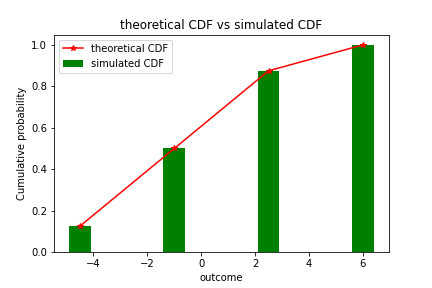
\includegraphics[width=9cm]{cdf.png}
    \caption{CDF}
\end{figure}
\begin{figure}[h!]
    \centering
    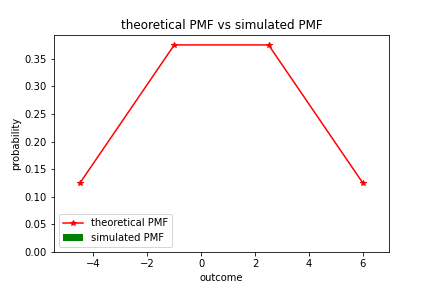
\includegraphics[width=9cm]{pmf.png}
    \caption{PMF}
\end{figure}
\section{Condition-2}
$X_{0}=Y$\\
$X_{1}=X_{0}+Y$\\
$X_{2}=X_{1}+X_{0}+Y$\\
\title\textbf{{There can be eight cases}}
\begin{enumerate}
    \item Case-\romannumeral1
    \begin{itemize}
        \item when $Z_{0}=0$,$Z_{1}=0$,$Z_{2}=0$\\
        \begin{align*}
            X_{0}&=-1.5\\
            X_{1}&=-1.5-1.5\\
            &=-3\\
            X_{2}&=-3-1.5-1.5\\
            &=-6
        \end{align*}
        \begin{align*}
            Pr(Z_{0}=0,Z_{1}=0,Z_{2}=0)&=\frac{1}{2}\times\frac{1}{2}\times\frac{1}{2}\\
            &=\frac{1}{8}
        \end{align*}
    \end{itemize}
    \item Case-\romannumeral2
    \begin{itemize}
        \item when $Z_{0}=0$,$Z_{1}=1$,$Z_{2}=1$\\
        \begin{align*}
            X_{0}&=-1.5\\
            X_{1}&=-1.5+2\\
            &=.5\\
            X_{2}&=-.5+-1.5+2\\
            &=1
        \end{align*}
        \begin{align*}
            Pr(Z_{0}=0,Z_{1}=1,Z_{2}=1)&=\frac{1}{2}\times\frac{1}{2}\times\frac{1}{2}\\
            &=\frac{1}{8}
        \end{align*}
    \end{itemize}
\newpage
     \item Case-\romannumeral3
    \begin{itemize}
        \item when $Z_{0}=0$,$Z_{1}=0$,$Z_{2}=1$\\
        \begin{align*}
            X_{0}&=-1.5\\
            X_{1}&=-1.5+-1.5\\
            &=-3\\
            X_{2}&=-3+-1.5+2\\
            &=-2.5
        \end{align*}
        \begin{align*}
            Pr(Z_{0}=0,Z_{1}=0,Z_{2}=1)&=\frac{1}{2}\times\frac{1}{2}\times\frac{1}{2}\\
            &=\frac{1}{8}
        \end{align*}
    \end{itemize}
    \item Case-\romannumeral4
    \begin{itemize}
        \item when $Z_{0}=1$,$Z_{1}=1$,$Z_{2}=1$\\
        \begin{align*}
            X_{0}&=2\\
            X_{1}&=2+2\\
            &=4\\
            X_{2}&=4+2+2\\
            &=8
        \end{align*}
        \begin{align*}
            Pr(Z_{0}=1,Z_{1}=1,Z_{2}=1)&=\frac{1}{2}\times\frac{1}{2}\times\frac{1}{2}\\
            &=\frac{1}{8}
        \end{align*}
    \end{itemize}
     \item Case-\romannumeral5
    \begin{itemize}
        \item when $Z_{0}=1$,$Z_{1}=0$,$Z_{2}=1$\\
        \begin{align*}
            X_{0}&=2\\
            X_{1}&=2-1.5\\
            &=.5\\
            X_{2}&=.5+2+2\\
            &=4.5
        \end{align*}
        \begin{align*}
            Pr(Z_{0}=1,Z_{1}=0,Z_{2}=1)&=\frac{1}{2}\times\frac{1}{2}\times\frac{1}{2}\\
            &=\frac{1}{8}
        \end{align*}
    \end{itemize}
     \item Case-\romannumeral6
    \begin{itemize}
        \item when $Z_{0}=1$,$Z_{1}=0$,$Z_{2}=0$\\
        \begin{align*}
            X_{0}&=2\\
            X_{1}&=2-1.5\\
            &=.5\\
            X_{2}&=.5+2+-1.5\\
            &=1
        \end{align*}
        \begin{align*}
            Pr(Z_{0}=1,Z_{1}=0,Z_{2}=0)&=\frac{1}{2}\times\frac{1}{2}\times\frac{1}{2}\\
            &=\frac{1}{8}
        \end{align*}
    \end{itemize}
    \item Case-\romannumeral7
    \begin{itemize}
        \item when $Z_{0}=1$,$Z_{1}=1$,$Z_{2}=0$\\
        \begin{align*}
            X_{0}&=2\\
            X_{1}&=2+2\\
            &=4\\
            X_{2}&=4+2+-1.5\\
            &=4.5
        \end{align*}
        \begin{align*}
            Pr(Z_{0}=1,Z_{1}=1,Z_{2}=0)&=\frac{1}{2}\times\frac{1}{2}\times\frac{1}{2}\\
            &=\frac{1}{8}
        \end{align*}
    \end{itemize}
    \item Case-\romannumeral8
    \begin{itemize}
        \item when $Z_{0}=0$,$Z_{1}=1$,$Z_{2}=0$\\
        \begin{align*}
            X_{0}&=-1.5\\
            X_{1}&=-1.5+2\\
            &=.5\\
            X_{2}&=.5+-1.5-1.5\\
            &=-2.5
        \end{align*}
        \begin{align*}
            Pr(Z_{0}=0,Z_{1}=1,Z_{2}=0)&=\frac{1}{2}\times\frac{1}{2}\times\frac{1}{2}\\
            &=\frac{1}{8}
        \end{align*}
    \end{itemize}
\end{enumerate}
\begin{table}[h!]
    \centering
    \begin{tabular}{|c|c|c|c|c|c|}
    \hline
         $X_{2}$&6&-2.5&1&4.5&8  \\[5pt]
         \hline
         $Pr(X_{2})$&$\frac{1}{8}$&$\frac{2}{8}$=$\frac{1}{4}$&$\frac{2}{8}$=$\frac{1}{4}$&$\frac{2}{8}$=$\frac{1}{4}$&$\frac{1}{8}$\\[5pt]
         \hline
    \end{tabular}
    \caption{Probability Distribution of $X_{2}$}
\end{table}
\begin{figure}[h!]
    \centering
    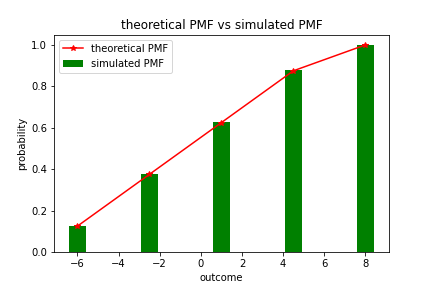
\includegraphics[width=9cm]{cdfnew.png}
    \caption{CDF}
\end{figure}
\begin{figure}[h!]
    \centering
    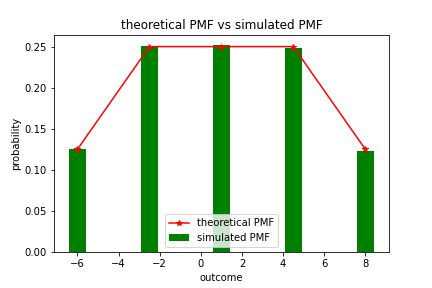
\includegraphics[width=9cm]{pdfnew.png}
    \caption{PMF}
\end{figure}
\end{document}
